\documentclass{article}

\usepackage{siunitx}
\usepackage{graphicx}
\usepackage{systeme}
\usepackage{amsmath}
\graphicspath{ {~/Desktop/} }

\author{Emanuele Casciaro}
\title{Presentazione algoritmo di Edit Distance}


\begin{document}
\maketitle
\tableofcontents

\newpage

\section{Introduzione}
In questo articolo verrà presentato l'algoritmo di Edit Distance, che date due stringhe $X$ e $Y$ ne restituisce la distanza di editing, ossia quante e quali operazioni effettuare per trasformare la prima nella seconda. Vedremo differenti approcci al problema e come essi influiscono sulle prestazioni

\section{Cenni teorici}
Seguirà ora una sezione contenente qualche cenno teorico, incentrato principalmente sull'aspetto d'interesse, ossia l'inferenza 

\subsection{Algoritmi Bottom Up}
L'Edit Distance è un algortimo di tipo Bottom Up, ciò vuol dire che la soluzione, a differenza degli algoritmi ricorsivi in coda (un famoso esempio è il calcolo del fattoriale), la soluzione viene calcolata a partire dai casi base, rendendo possibile calcolare successivamente il risultato generale.

\section{Edit Distance: risoluzione}
Costruiamo adesso la soluzione di un generico problema, esaminando caso base e caso generico.
In seguito verrà usata la notazione $S_i$ per indicare il prefisso lungo $i$ della stringa $S$, e $si$ per indicarne il suo $i$-esimo carattere.\newline
Essendo l'algoritmo di tipo bottom-up, arrivati al passo $i$, è nota la distanza di editing per le sottostringhe $X_{i-1}$ e $Y_{i-1}$\newline
Si calcolano quindi i costi di tutte le sottostringhe, che andranno allora a formare una matrice $m \times n$, dove $m = |X|$ e $n = |Y|$
\subsection{Operazioni ammesse}
Le operazioni eseguibili su una stringa considerate sono le seguenti:
\begin{itemize}
	\item Inserimento (\emph{costo 1}): se $|X| < |Y|$ aggiungo ad $X$ i caratteri mancanti.
	\item Cancellazione (\emph{costo 1}): se $|X| > |Y|$ elimino da $X$ i caratteri non necessari.
	\item Copia (\emph{costo 0}): se $x_i = y_j$ non devo eseguire modifiche, e passo al passo successivo.
	\item Sostituzione (\emph{costo 1}): se $x_i \ne y_j$ sostituisco il carattere sbagliato; tale processo può essere visto come una cancellazione ed un inserimento.
	\item Scambio (\emph{costo 1}): se $x_i = y_{j-1}$ e $x_{i-1} = y_i$ inverto il carattere $x_i$ ed il carattere $x_{i-1}$.
\end{itemize}
Nota: i costi assegnati sono molto semplificati, e non tengono considerazione di fattori quali la vicinanza delle lettere o eventuali errori di battitura.

\subsection{Caso base: $X$ o $Y$ è una stringa vuota}
Se $Y$ è una stringa vuota, basterà eseguire $|Y|$ rimozioni in $X$ per ottenere due stringhe uguali; viceversa, se ad essere vuota è $X$, eseguo $|Y|$ inserimenti. Allora si andranno a calcolare tutti i costi $$c_{1, j} \forall j \in [1, n+1]$$$$  c_{(, 1} \forall i \in [1, m+1]$$

\subsection{Caso generico: $X$ e $Y$ stringhe non vuote}
In questo caso, applico le varie operazioni, sommando il loro costo all'adeguato sottocaso:


$$
c_{i, j}=\begin{cases} c_{i-1. j-1} + costo(copia) \\ c_{i-1. j-1} + costo(sostituzione) \\  c_{i-2. j-2} + costo(scambio) \\ c_{i-1. j} + costo(cancellazione) \\ c_{i. j-1} + costo(inserimento) \end{cases}
$$
 A questo punto itero per tutti gli indici, giungendo eventualmente a $c_{m+1, n+1}$, la soluzione del problema originale.
 
 \section{Indice di Jaccard}
 Un uso realistico dell'algoritmo è nella correzione di eventuali errori di battitura: si compara la stringa inserita con un vocabolario, e si restituisce le stringhe più vicine. Sorge, al crescere del vocabolario, un problema prestazionale. Infatti è inutile eseguire l'algoritmo su tutti gli elementi del vocabolario, la maggiora parte infatti non ha nulla in comune con la stringa inserita. \newline
 Si prendono allora le stringhe con elevato \emph{Indice di Jaccard}, ossia $$JC = \frac{|X \cap Y| }{|X \cup Y|}$$
 Dove, in generela, $X$ è l'insieme degli \emph{n-grammi} della stringa, ossia tutte le sottostringhe distinte lunghe $n$ contenute in essa.
Ovviamente se $JC = 1$ le parole coincidono.
 
\section{Test}
Il programma realizzato evidenzia come l'uso dell'Indice di Jaccard influisca sulle performance. 
Verranno prese in considerazione una serie di parole appartenenti al lessico di partenza, che dopo una serie di permutazioni delle lettere (simulo un typo) verranno confrontate con il lessico stesso. Sulle stesse stringhe verrà eseguito l'algoritmo in entrambe le versioni, con e senza indice di Jaccard (il test di Jaccard è eseguito in configurazione: $threshold = 0.33$ e con una suddivisione in bi-grammi, ossia n-grammi con $n=2$) \newline
Entrambi gli approcci verranno poi confrontati, paragonando i tempi di esecuzione.

\section{Risultati attesi}
Data la mole di stringhe nel lessico, è lecito aspettarci un tempo di esecuzione molto maggiore nel caso in cui non si usi l'indice di Jaccard, dato che ciò comporta l'assenza totale di qualsivoglia filtro per le parole troppo differenti. \newline 
Questi tempi dovrebbero ridursi ulteriormente al crescere del valore di $threshold$, che rende il filtro sempre più rigido.
\newpage
\section{Risultati e conclusioni}

\begin{figure}[h]
\centering
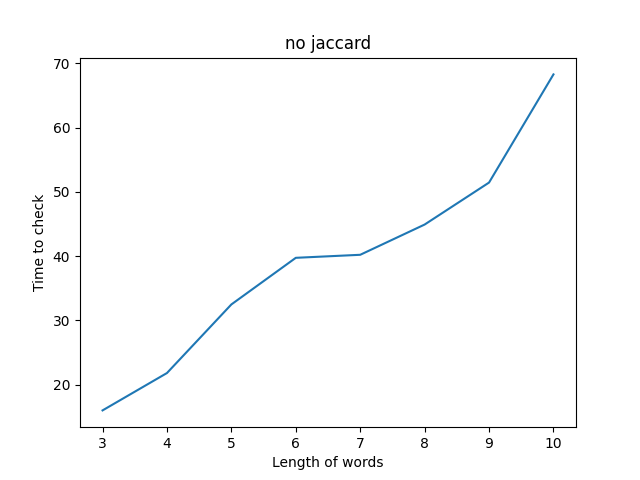
\includegraphics[width=0.7\linewidth]
{"./myplotnj.png"}
\label{no jaccard}
\end{figure}
\begin{figure}[h]
\centering
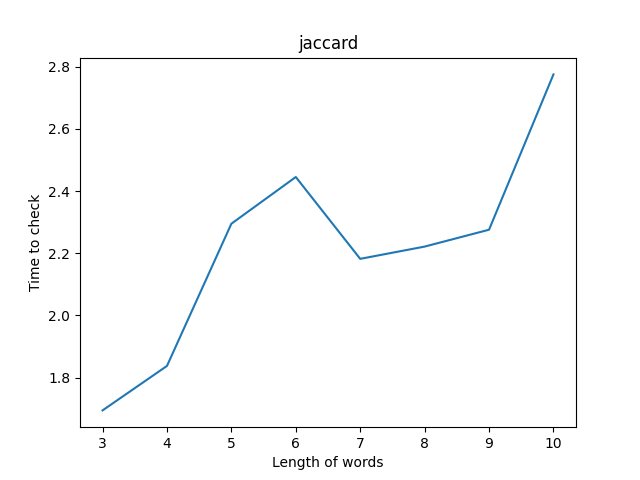
\includegraphics[width=0.7\linewidth]
{"./myplotj.png"}
\label{jaccard}
\end{figure}
Alla fine i test hanno rivelato i risultati pronosticati: una possibile ulteriore conferma di questo trend è considerare cosa succedere al crescere del minimo indice di Jaccard richiesto; infatti se si richiedesse una precisionie del 100\% l'algoritmo restituirebbe soltato un eventuale stringa identica (riducendo così l'algoritmo ad un banale algoritmo di ricerca), scartando praticamente ogni stringa (con quindi esecuzione rapida e pochi match).
\newpage
\begin{figure}[h]
\centering
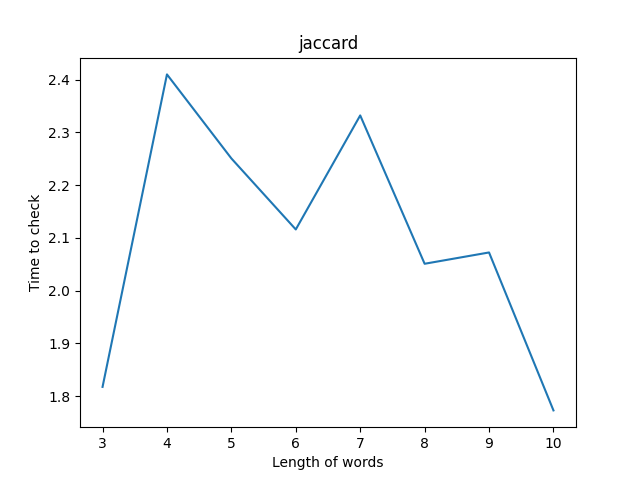
\includegraphics[width=0.7\linewidth]
{"./myplotj66.png"}
\label{jaccard (threshold=0.66)}
\end{figure}
Si può però notare un comportamento diverso al variare del valore di soglia (terzo grafico ha soglia a 0.66), che abbassa i tempi di esecuzione come previsto, ma con un effetto più apprezzabile con le parole più lunghe, facendo venire meno quell'apparente relazione di linearità che appare se non si usa l'indice di Jaccard o se lo si usa con soglia bassa
	

\end{document}